% Chapter Template

\chapter{Analytic Results} % Main chapter title

\label{Chapter4} % Change X to a consecutive number; for referencing this chapter elsewhere, use \ref{ChapterX}

\lhead{Chapter 4. \emph{Analytic Results}} % Change X to a consecutive number; this is for the header on each page - perhaps a shortened title

%----------------------------------------------------------------------------------------
%	SECTION: INTRO
%----------------------------------------------------------------------------------------

\section{Introduction}
In this chapter we present results obtained using stochastic collocation for generalized polynomial chaos
expansions (SCgPC) and high-dimension model reduction (HDMR) uncertainty quantification methods.  In each case
we also include Monte Carlo as a comparison benchmark.

Our primary objective in expanding the usability of collocation-based methods is to reduce the number of
computational model solves necessary to obtain reasonable second-order statistics for the model.  For each
analytic model described in Chapter \ref{Chapter3}, we present value figures and convergence figures.  

Value figures show the values of the mean or standard deviation obtained, along with the benchmark analytic
value as a dotted line.  The Monte Carlo samples are taken at a few select points.  Error bars are provided
for the Monte Carlo method and are estimated using the population variance,
\begin{equation}
  \epsilon_{95} = \frac{1.96\bar\sigma_N}{\sqrt{N}},
\end{equation}
\begin{equation}
  \bar\sigma_N^2 = \frac{N}{N-1}\sigma^2_N = \frac{N}{N-1}\qty(\frac{1}{N}\sum_{i=1}^M u(Y_i)^2 - \bar
  u(Y)^2_N),
\end{equation}
where $Y_i$ are a set of $M$ independent identically-distributed realizations taken from the input space.
These errorbars estimate where the value of the statistic is with a probability near 0.95.  The estimate of
this error improves as additional samples are taken.

Convergence figures are
log-log error graphs with the number of computational solves on the x-axis and error with the analytical
solution on the y-axis.  The distinct lines demonstrate series of results obtained for each UQ method.  Each
series obtains additional values by increasing the refinement of the method.  For Monte Carlo, additional
samples are added.  For static SCgPC, higher-order polynomials are used in the representative expansion.  For
adaptive methods, additional solves are allowed to adaptively include additional polynomials and/or dimension
subsets.

The measure of success for a method is less dependent on the absolute value of the error shown.  Instead, the
rate of convergence as refinement increases determines the desirability of the method for that model.  We
expect the rate of convergence to depend on two factors: the dimensionality of the uncertain space for the
model, and the continuity of the response measured.  We consider the convergence of both the mean and the
standard deviation for each model.

The series considered include analog Monte Carlo (mc), Tensor Product polynomial expansion construction method
(tp), Total Degree polynomial expansion construction method (td), Hyperbolic Cross polynomial expansion
construction method (hc), adaptive sparse grid collocation for generalized polynomial chaos expansion
(adaptSC), and adaptive HDMR or adaptive Sobol decomposition (adaptSobol).

We additionally note that results from \raven{} computations were written to file using 10 digits of accuracy.
As a result, any apparent convergence past this level of accuracy is coincidental or the result of
machine-exact values, and we consider a relative difference of $10^{-10}$ to be converged.

\section{Tensor Monomials}
This model is described in section \ref{mod:first tensor poly}.  As this polynomial contains only combinations of
first-order polynomials, we expect the Tensor Product index set construction method (TP) to be very efficient
in absolute error magnitude.  Because the model has infinite continuity, we expect all collocation-based
methods to be quite efficient.  The values and errors of the mean and standard deviation are given in Figures
\ref{fig:tensormono mean values 5} through \ref{fig:tensormono var errors 5} for 5 uncertain inputs, and the same
for 10 dimensions is given in Figures \ref{fig:tensormono mean values 10} through \ref{fig:tensormono var
errors 10}.  Note that TP exactly reproduces the original model with expansion order 1, so no convergence is
observed past the initial sampling point.

\subsection{3 Inputs}
The strength of collocation methods is clear for this small-dimensionality problem of three uncertain inputs.
The convergence on the
mean and standard deviation is swift for all the methods.  Both adaptive methods converge at nearly identical
rates; this is not surprising, as for small dimension problems the adaptive search follows a very similar
path.
\begin{figure}[H]
  \centering
  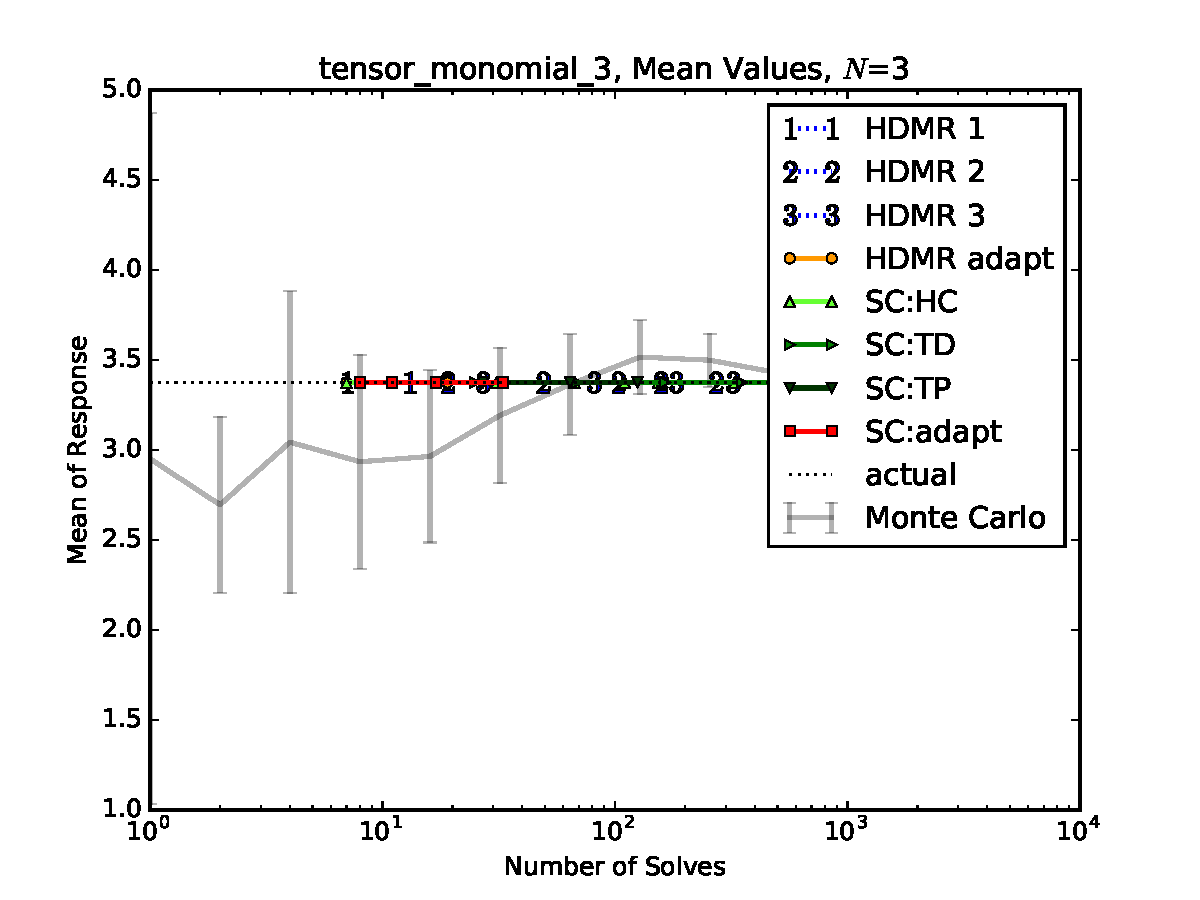
\includegraphics[width=0.7\linewidth]{anlmodels/tensor_monomial_3_mean_vals}
  \caption{Tensor Monomial, $N=3$, Mean Values}
  \label{fig:tensormono mean values 3}
\end{figure}
\begin{figure}[H]
  \centering
  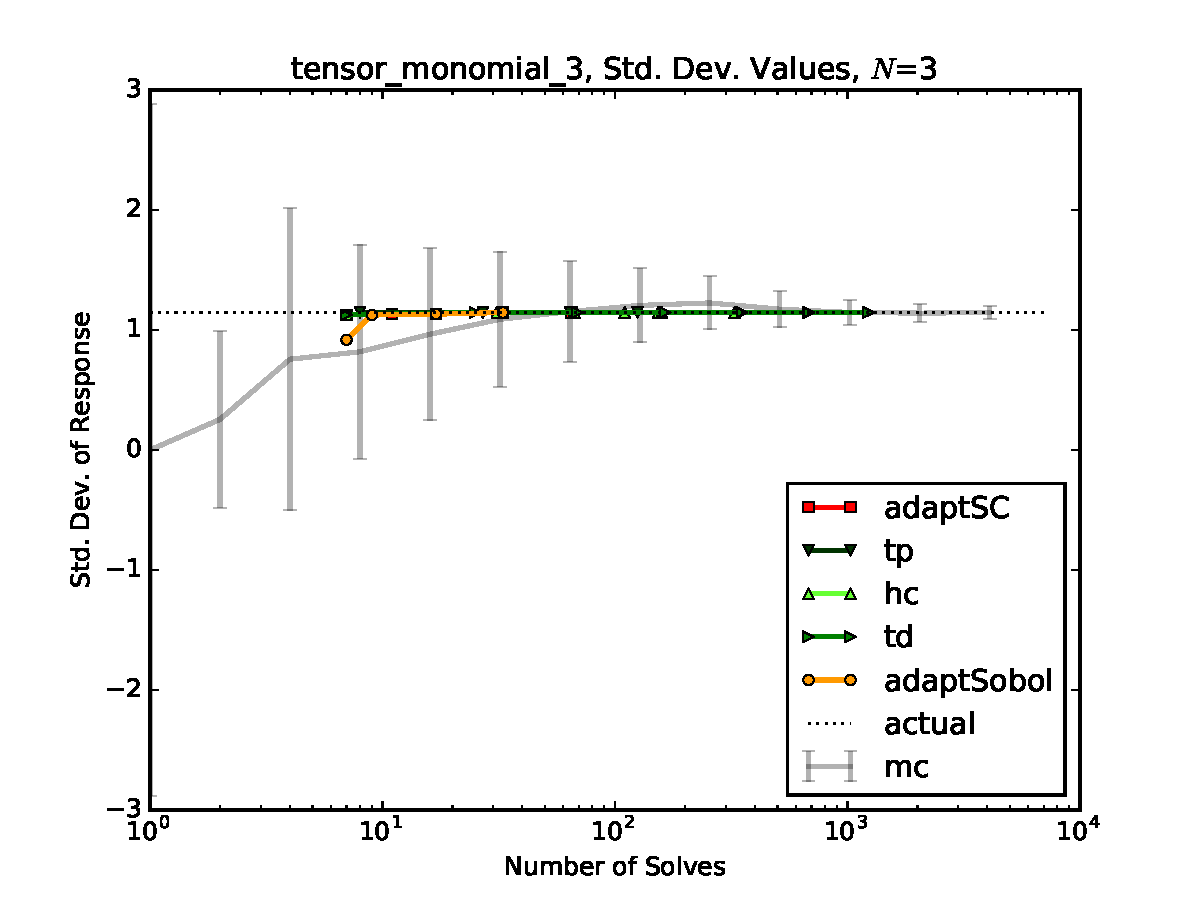
\includegraphics[width=0.7\linewidth]{anlmodels/tensor_monomial_3_var_vals}
  \caption{Tensor Monomial, $N=3$, Std. Dev. Values}
  \label{fig:tensormono var values 3}
\end{figure}

\begin{figure}[H]
  \centering
  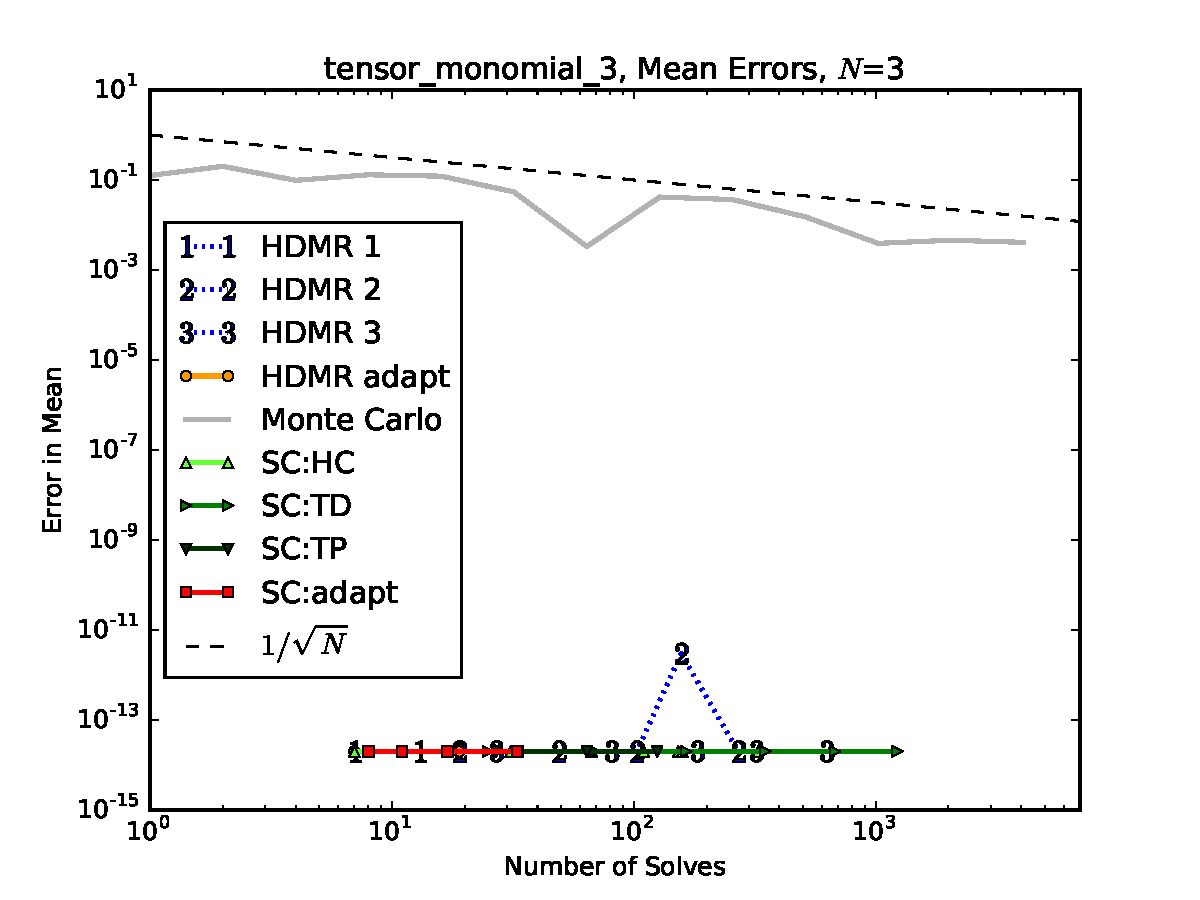
\includegraphics[width=0.7\linewidth]{anlmodels/tensor_monomial_3_mean_errs}
  \caption{Tensor Monomial, $N=3$, Mean Convergence}
  \label{fig:tensormono mean errors 3}
\end{figure}
\begin{figure}[H]
  \centering
  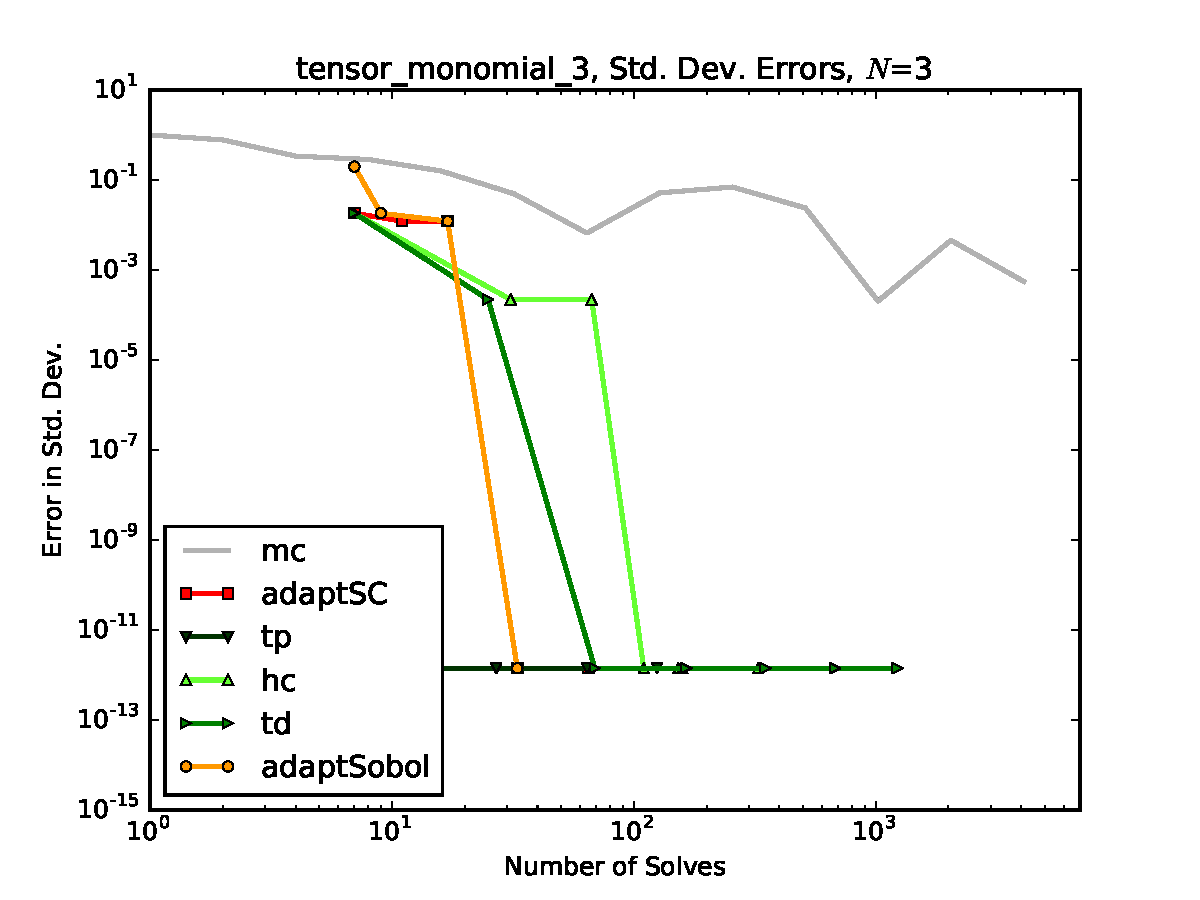
\includegraphics[width=0.7\linewidth]{anlmodels/tensor_monomial_3_variance_errs}
  \caption{Tensor Monomial, $N=3$, Std. Dev. Convergence}
  \label{fig:tensormono var errors 3}
\end{figure}




\subsection{5 Inputs}
While the convergence on the mean is still direct for the five-dimensional input problem, we begin to see
degradation in the convergence of collocation-based methods.  Total Degree outperforms adaptive methods, as
the search algorithms struggle to find the optimal tensors of low-order polynomials required.  Hyperbolic
Cross is outperformed by Total Degree, as expected for a problem with this level of regularity.
\begin{figure}[H]
  \centering
  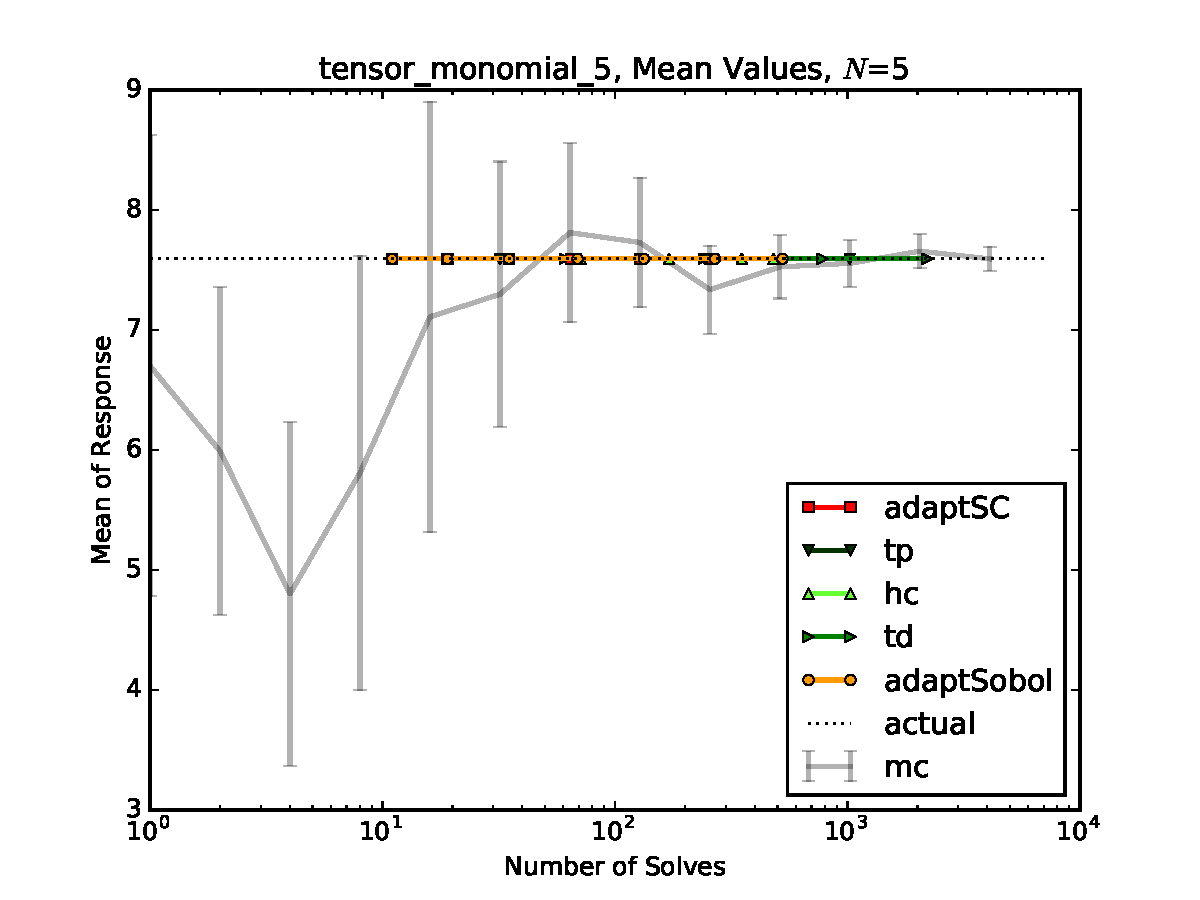
\includegraphics[width=0.7\linewidth]{anlmodels/tensor_monomial_5_mean_vals}
  \caption{Tensor Monomial, $N=5$, Mean Values}
  \label{fig:tensormono mean values 5}
\end{figure}
\begin{figure}[H]
  \centering
  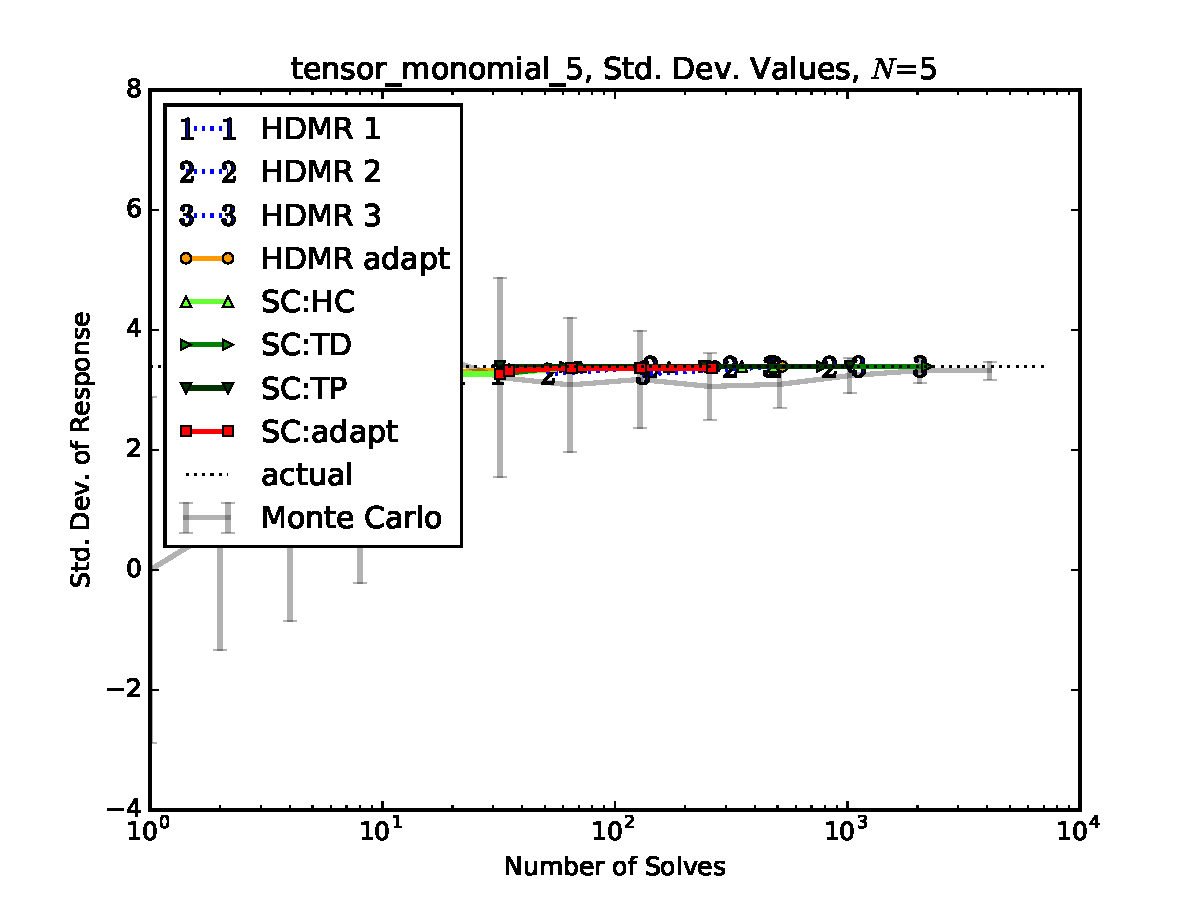
\includegraphics[width=0.7\linewidth]{anlmodels/tensor_monomial_5_var_vals}
  \caption{Tensor Monomial, $N=5$, Std. Dev. Values}
  \label{fig:tensormono var values 5}
\end{figure}

\begin{figure}[H]
  \centering
  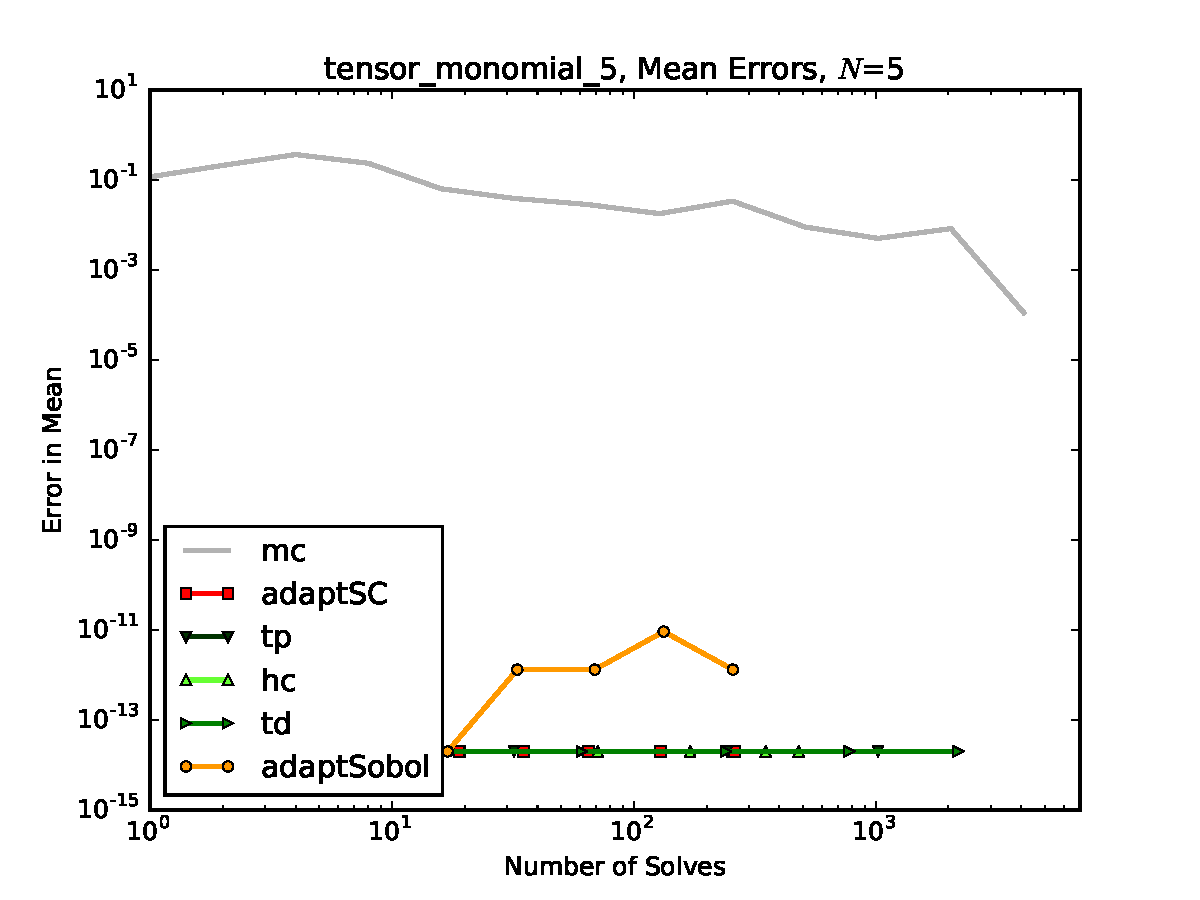
\includegraphics[width=0.7\linewidth]{anlmodels/tensor_monomial_5_mean_errs}
  \caption{Tensor Monomial, $N=5$, Mean Convergence}
  \label{fig:tensormono mean errors 5}
\end{figure}
\begin{figure}[H]
  \centering
  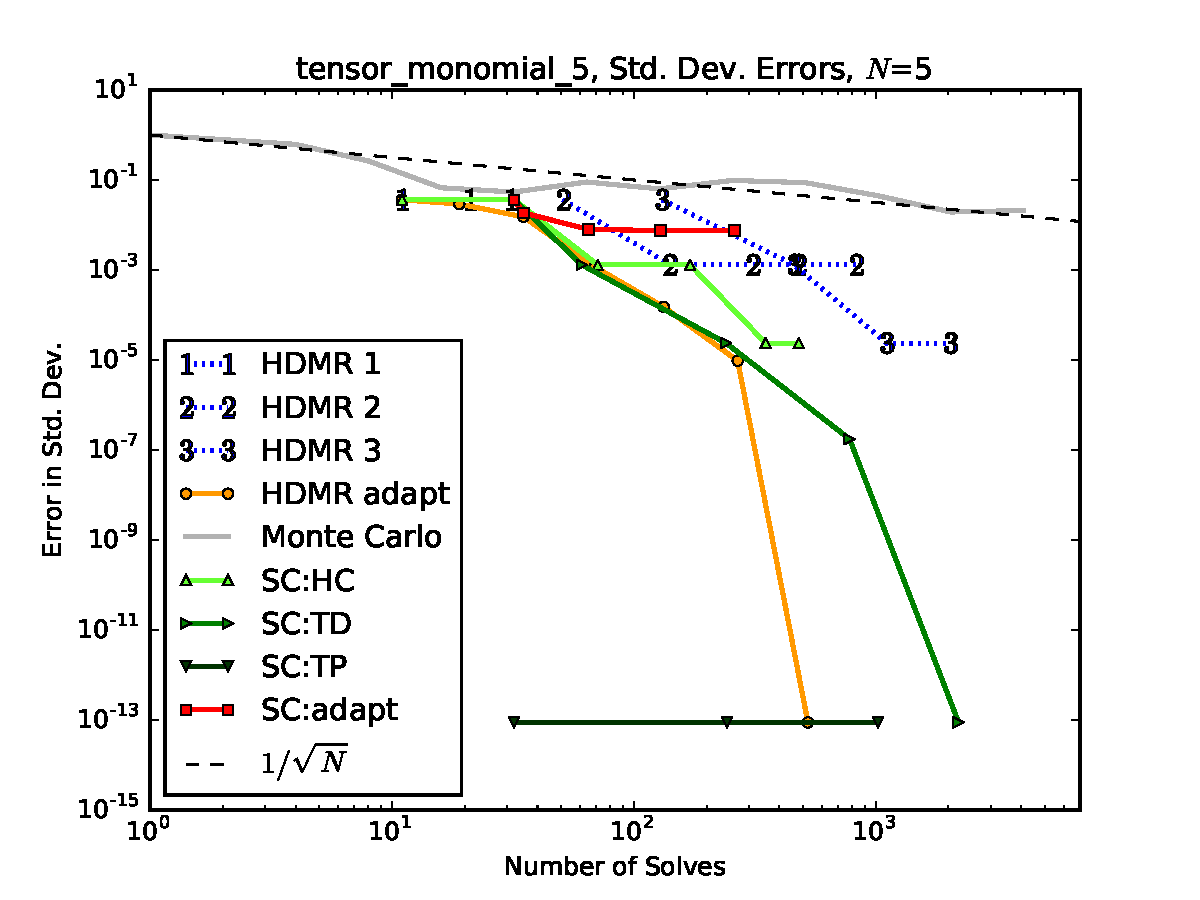
\includegraphics[width=0.7\linewidth]{anlmodels/tensor_monomial_5_variance_errs}
  \caption{Tensor Monomial, $N=5$, Std. Dev. Convergence}
  \label{fig:tensormono var errors 5}
\end{figure}

\subsection{10 Inputs}
As we increase to ten inputs, we see significant degradation of all the collocation methods in converging on
the standard deviation.  While it appears there is exponential convergence, the curvature is quite large, and
little better than linear convergence is observed for up to 1000 computational solves.  One reason the
adaptive methods do not perform more admirably for this case is the equal-weight importance of all the input
terms as well as the polynomial terms; the high-dimensional space takes considerable numbers of runs to
explore thoroughly, and this model contains some of the most difficult polynomials to find adaptively: those including
all of the inputs. 
\begin{figure}[H]
  \centering
  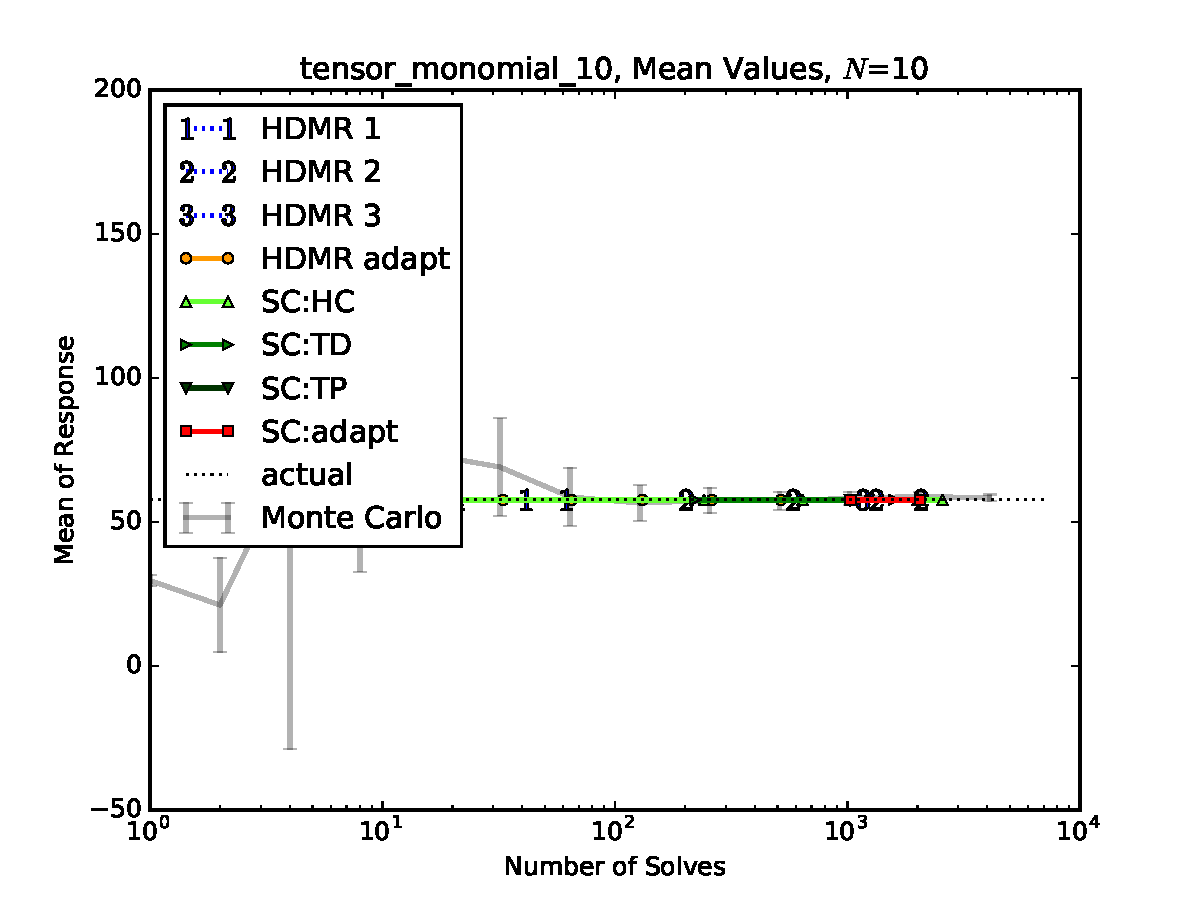
\includegraphics[width=0.7\linewidth]{anlmodels/tensor_monomial_10_mean_vals}
  \caption{Tensor Monomial, $N=10$, Mean Values}
  \label{fig:tensormono mean values 10}
\end{figure}
\begin{figure}[H]
  \centering
  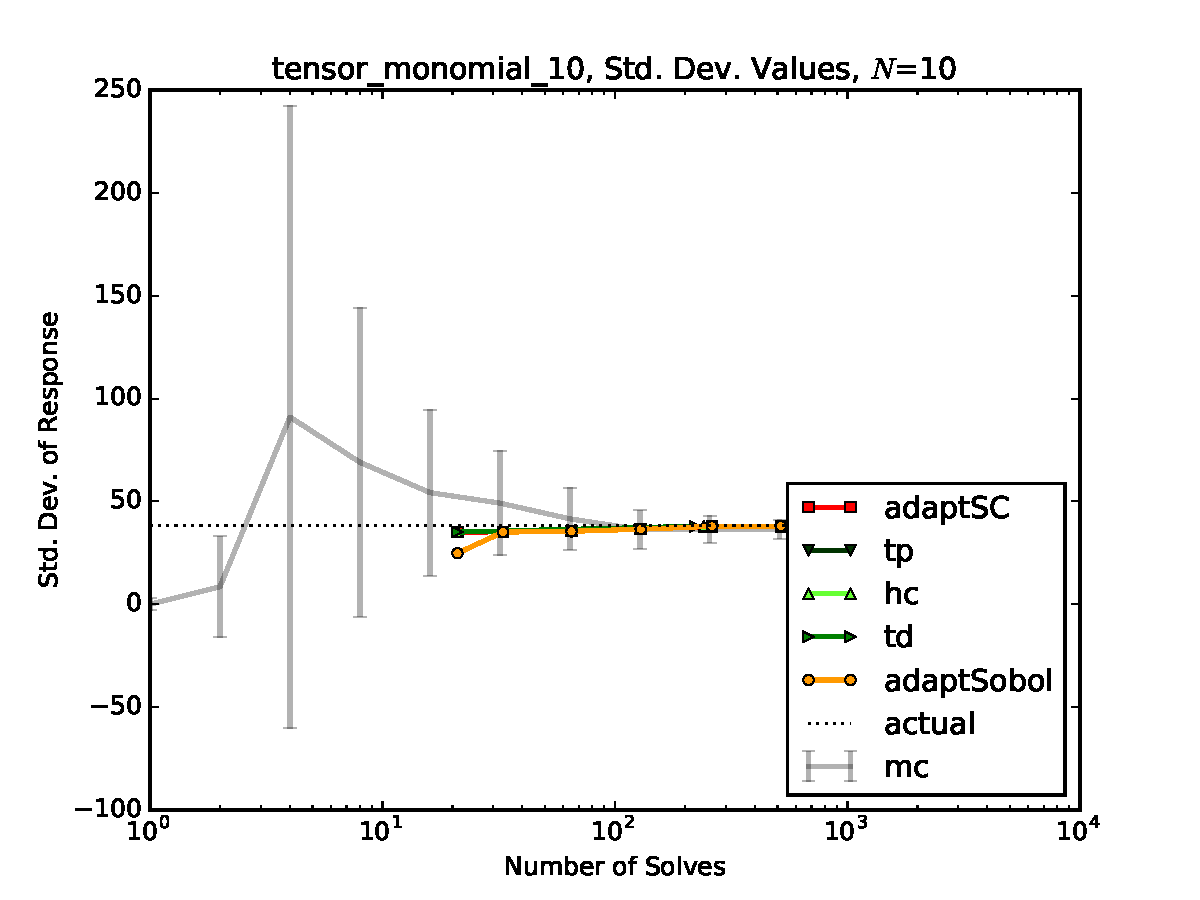
\includegraphics[width=0.7\linewidth]{anlmodels/tensor_monomial_10_var_vals}
  \caption{Tensor Monomial, $N=10$, Std. Dev. Values}
  \label{fig:tensormono var values 10}
\end{figure}

\begin{figure}[H]
  \centering
  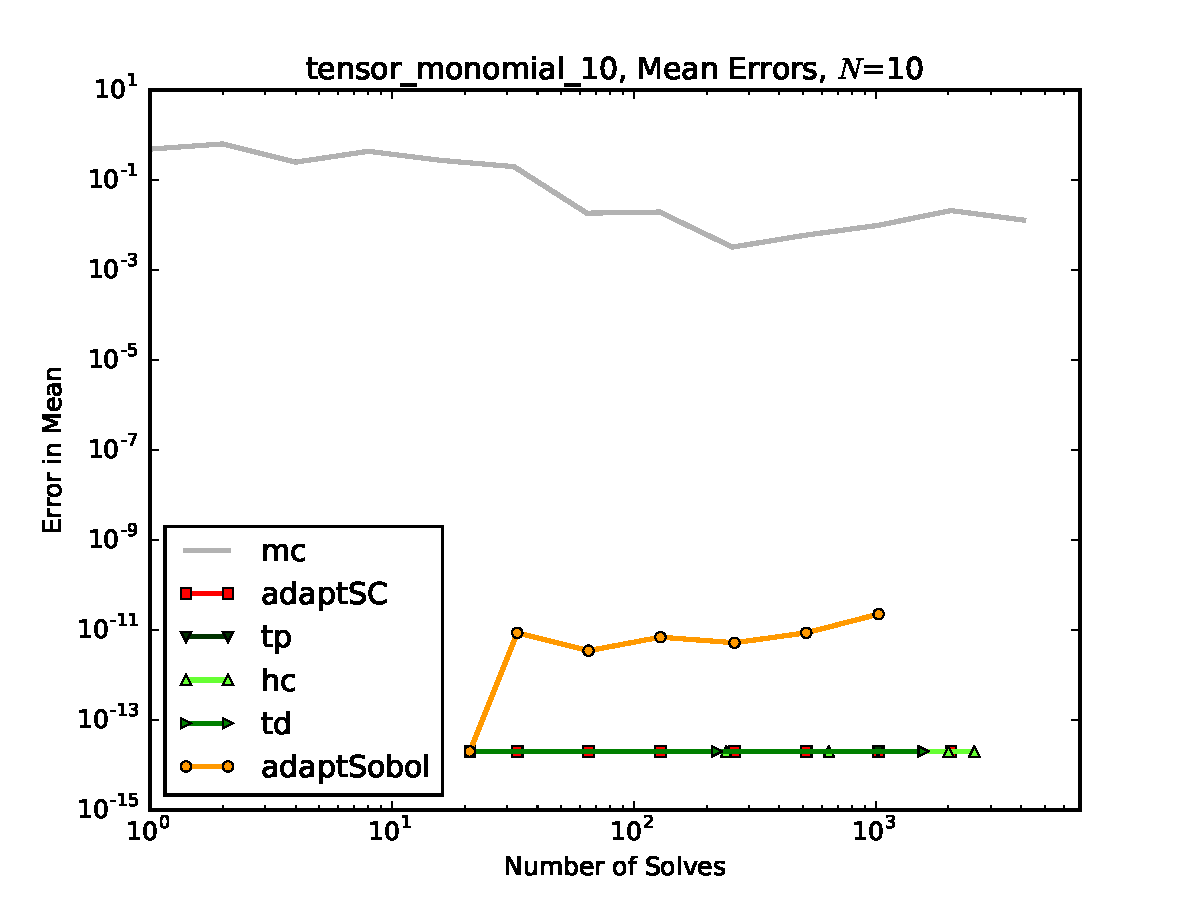
\includegraphics[width=0.7\linewidth]{anlmodels/tensor_monomial_10_mean_errs}
  \caption{Tensor Monomial, $N=10$, Mean Convergence}
  \label{fig:tensormono mean errors 10}
\end{figure}
\begin{figure}[H]
  \centering
  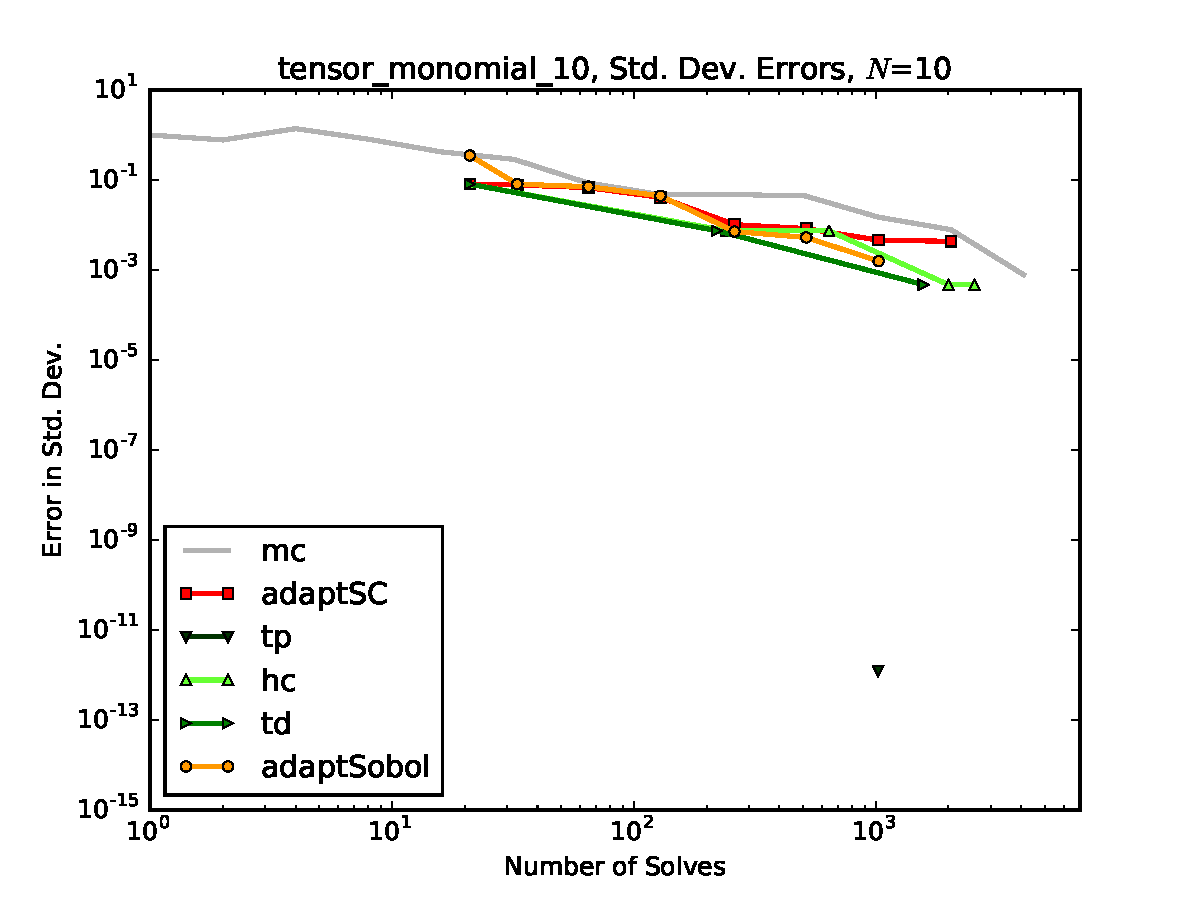
\includegraphics[width=0.7\linewidth]{anlmodels/tensor_monomial_10_variance_errs}
  \caption{Tensor Monomial, $N=10$, Std. Dev. Convergence}
  \label{fig:tensormono var errors 10}
\end{figure}


\section{Sudret Polynomial}
This model is described in section \ref{mod:sudret}.

\subsection{3 Inputs}
\begin{figure}[H]
  \centering
  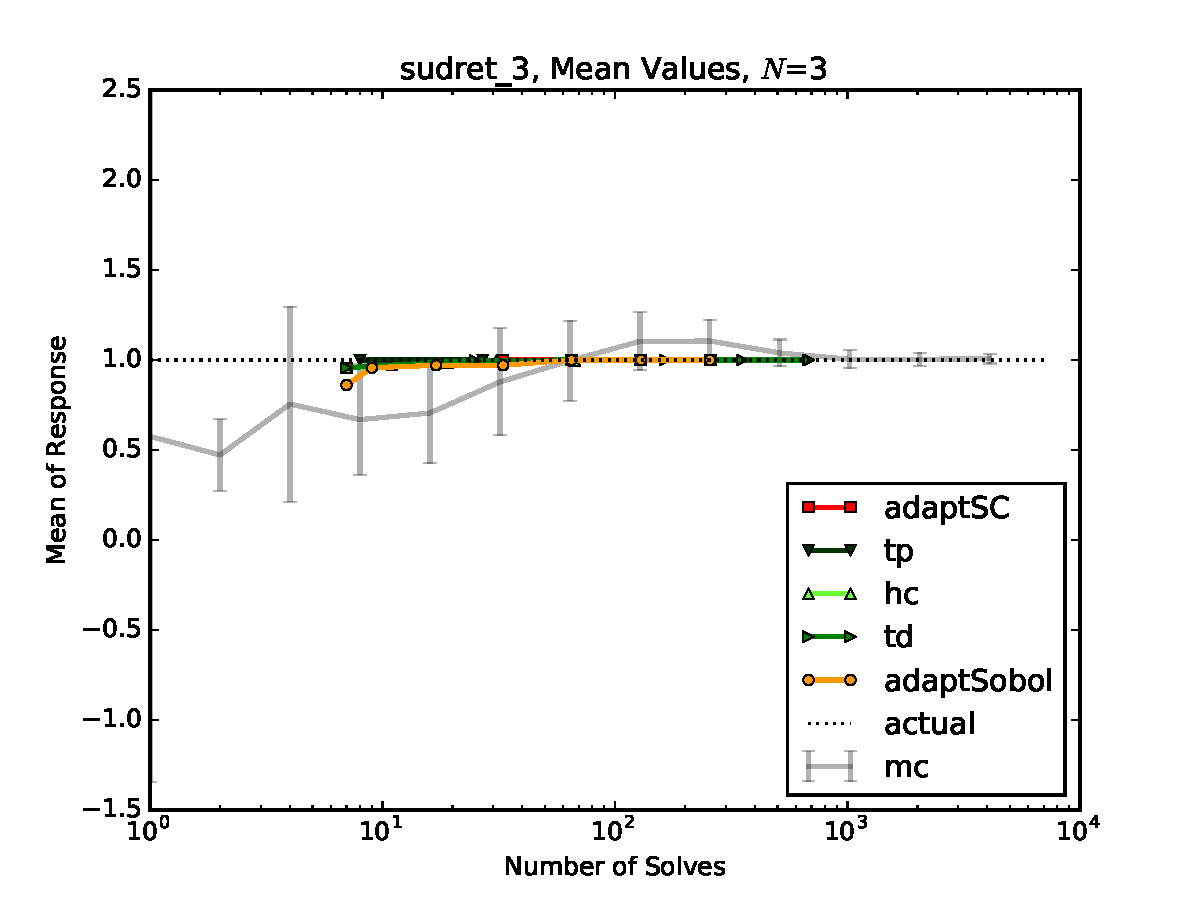
\includegraphics[width=0.7\linewidth]{anlmodels/sudret_3_mean_vals}
  \caption{Sudret Polynomial, $N=3$, Mean Values}
  \label{fig:sudretpoly mean values 3}
\end{figure}
\begin{figure}[H]
  \centering
  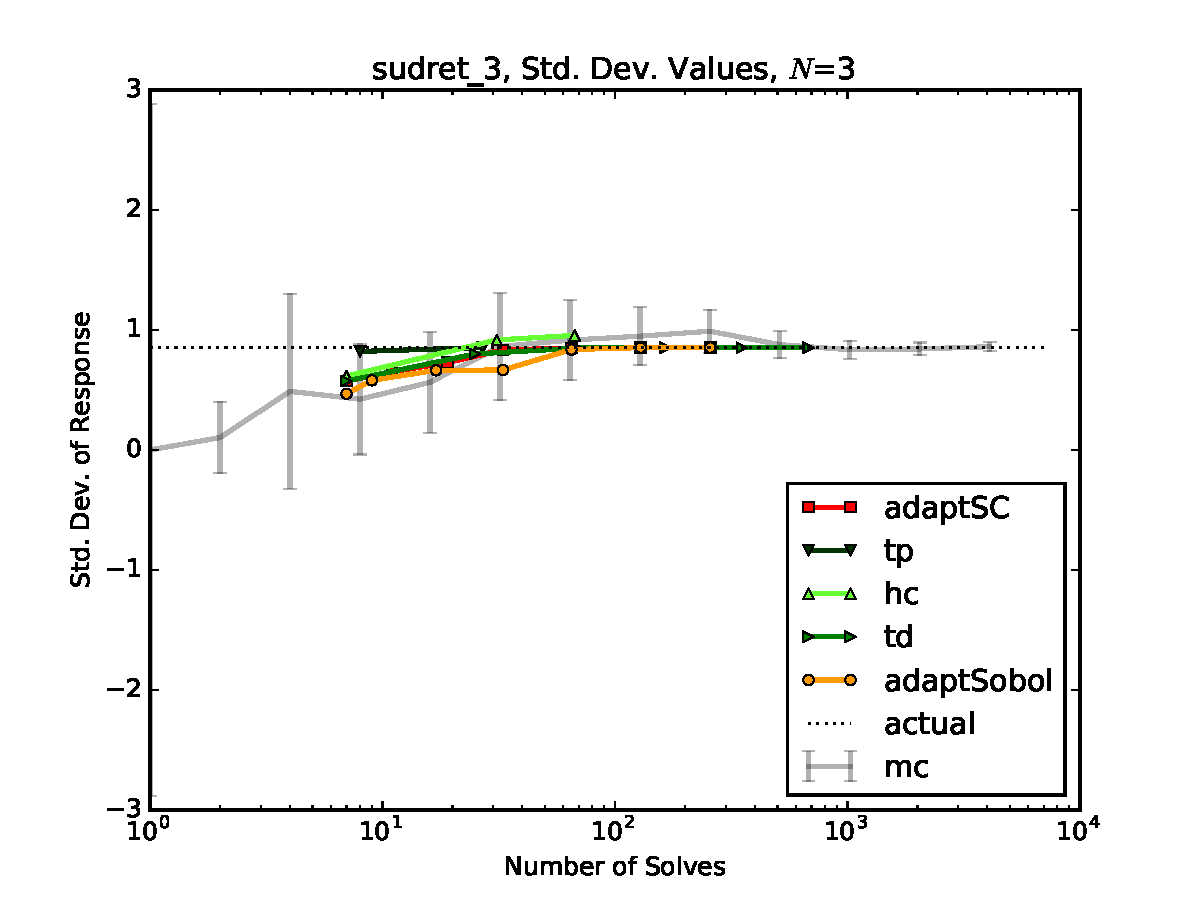
\includegraphics[width=0.7\linewidth]{anlmodels/sudret_3_var_vals}
  \caption{Sudret Polynomial, $N=3$, Std. Dev. Values}
  \label{fig:sudretpoly var values 3}
\end{figure}

\begin{figure}[H]
  \centering
  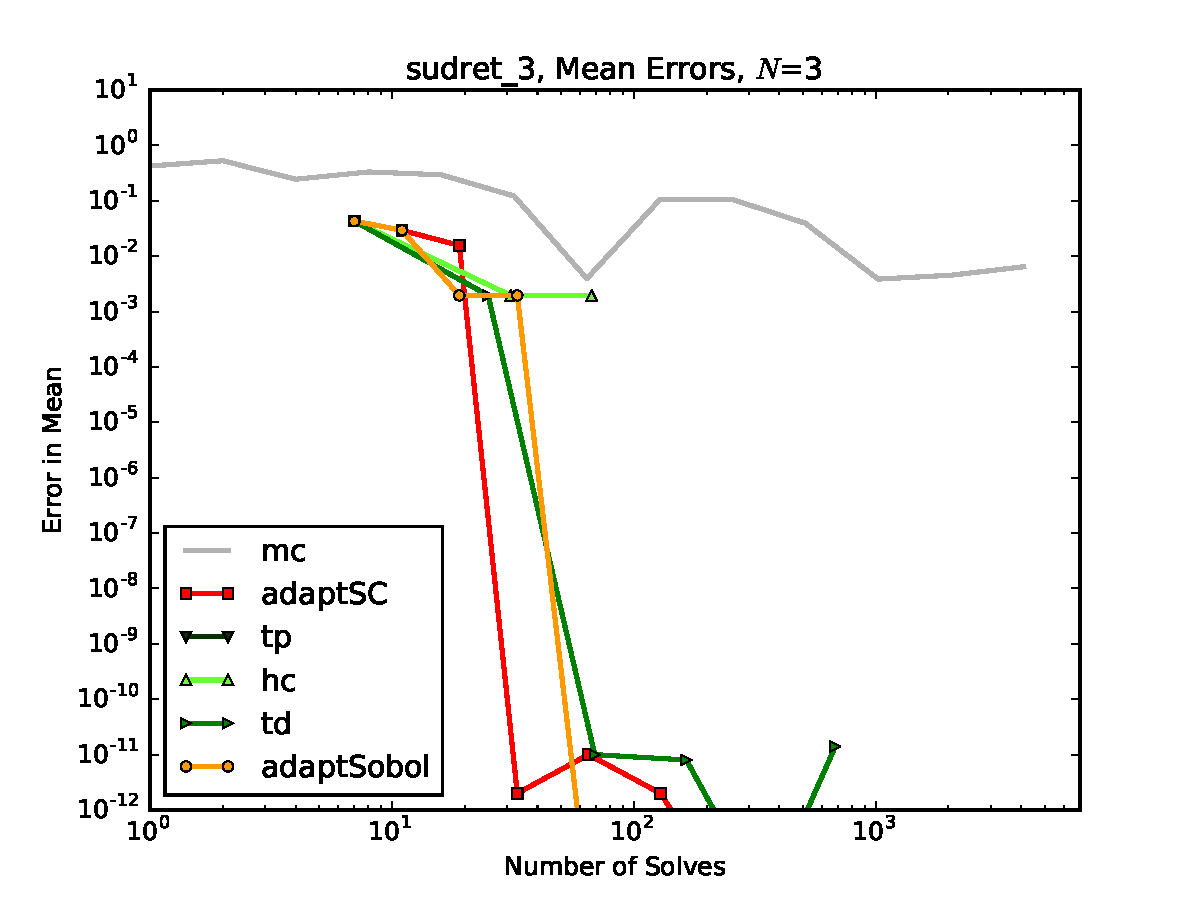
\includegraphics[width=0.7\linewidth]{anlmodels/sudret_3_mean_errs}
  \caption{Sudret Polynomial, $N=3$, Mean Convergence}
  \label{fig:sudretpoly mean errors 3}
\end{figure}
\begin{figure}[H]
  \centering
  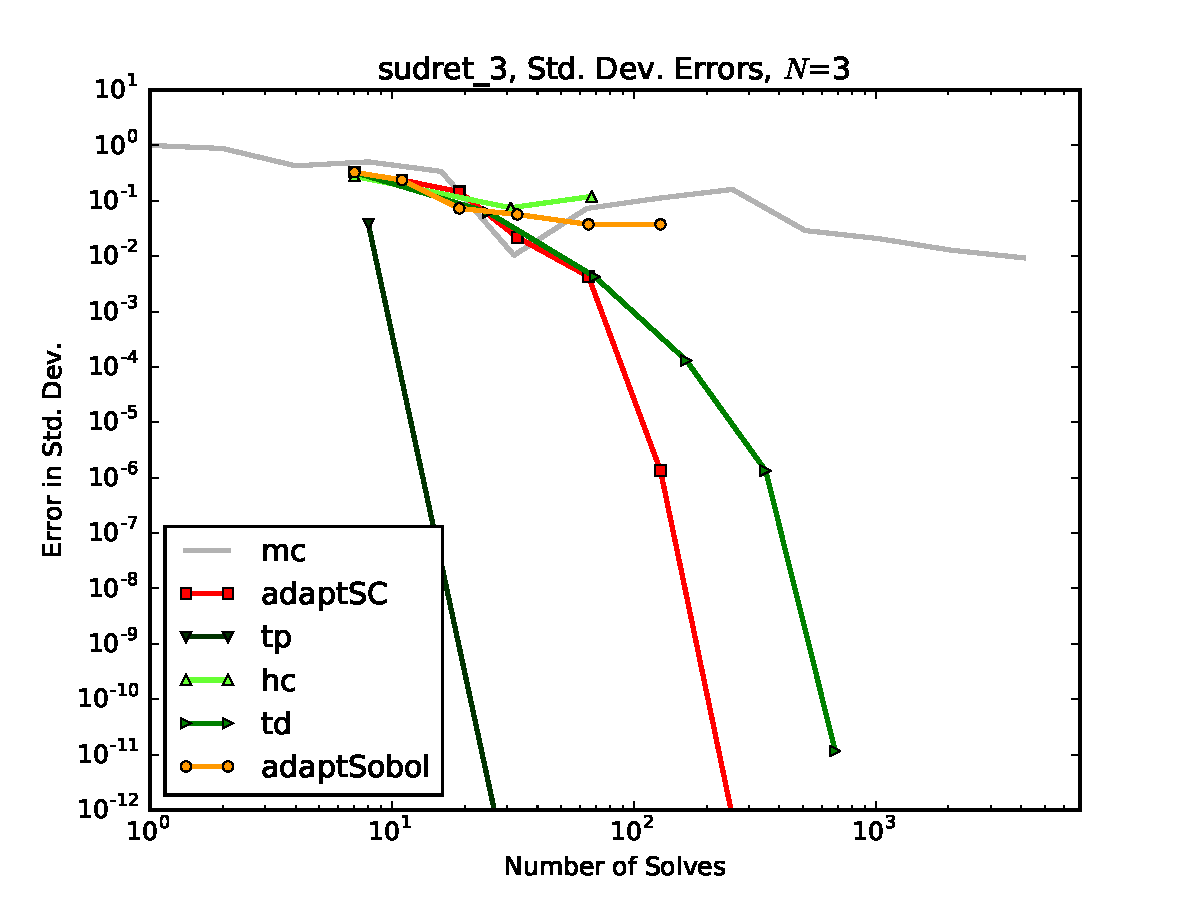
\includegraphics[width=0.7\linewidth]{anlmodels/sudret_3_variance_errs}
  \caption{Sudret Polynomial, $N=3$, Std. Dev. Convergence}
  \label{fig:sudretpoly var errors 3}
\end{figure}

\subsection{5 Inputs}
\begin{figure}[H]
  \centering
  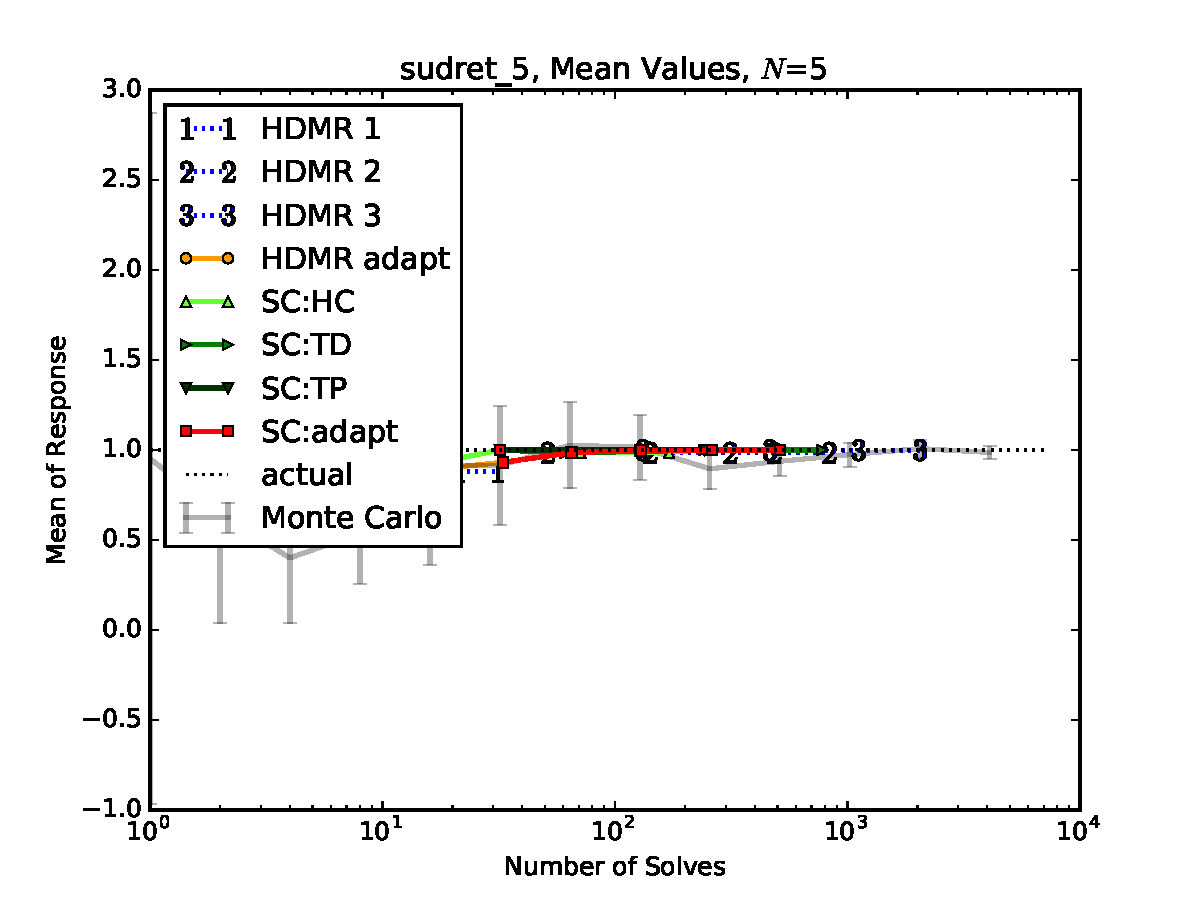
\includegraphics[width=0.7\linewidth]{anlmodels/sudret_5_mean_vals}
  \caption{Sudret Polynomial, $N=5$, Mean Values}
  \label{fig:sudretpoly mean values 5}
\end{figure}
\begin{figure}[H]
  \centering
  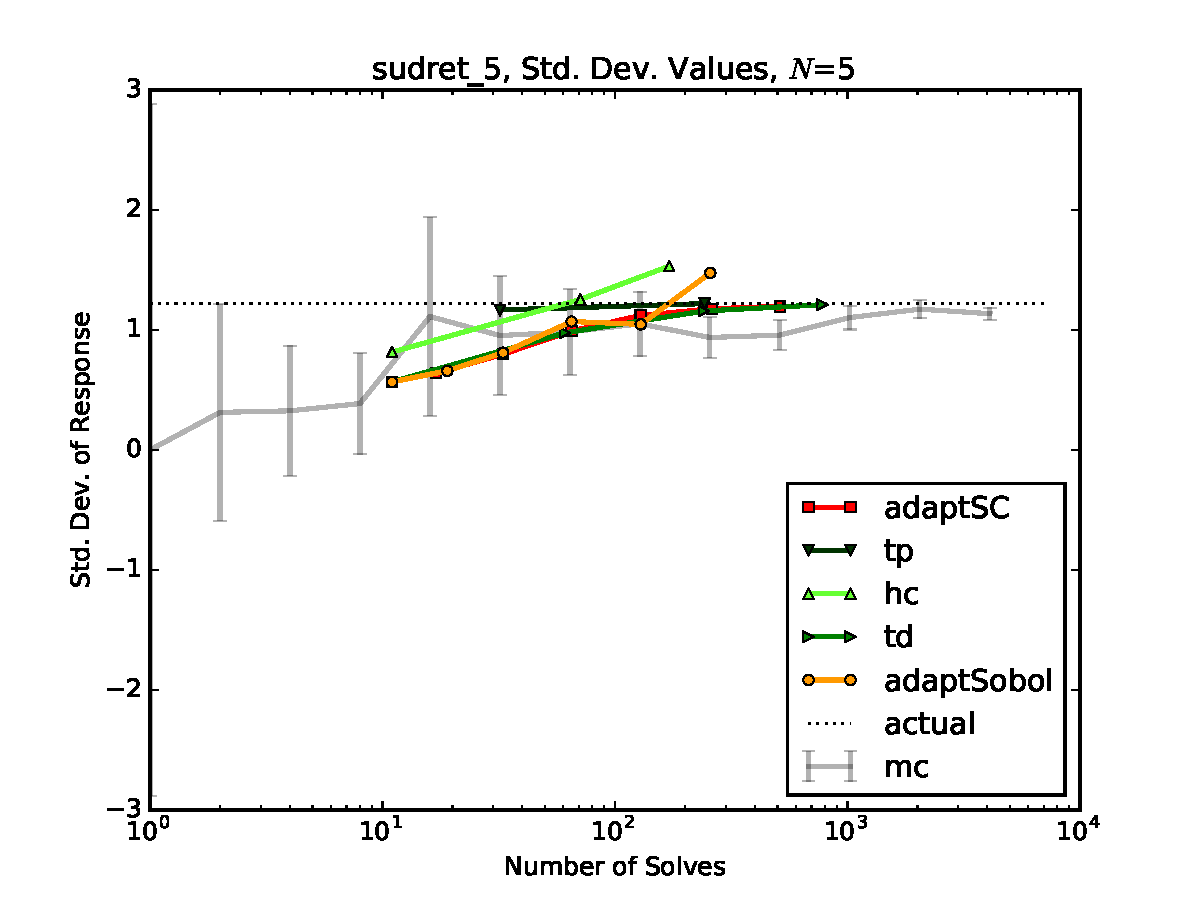
\includegraphics[width=0.7\linewidth]{anlmodels/sudret_5_var_vals}
  \caption{Sudret Polynomial, $N=5$, Std. Dev. Values}
  \label{fig:sudretpoly var values 5}
\end{figure}

\begin{figure}[H]
  \centering
  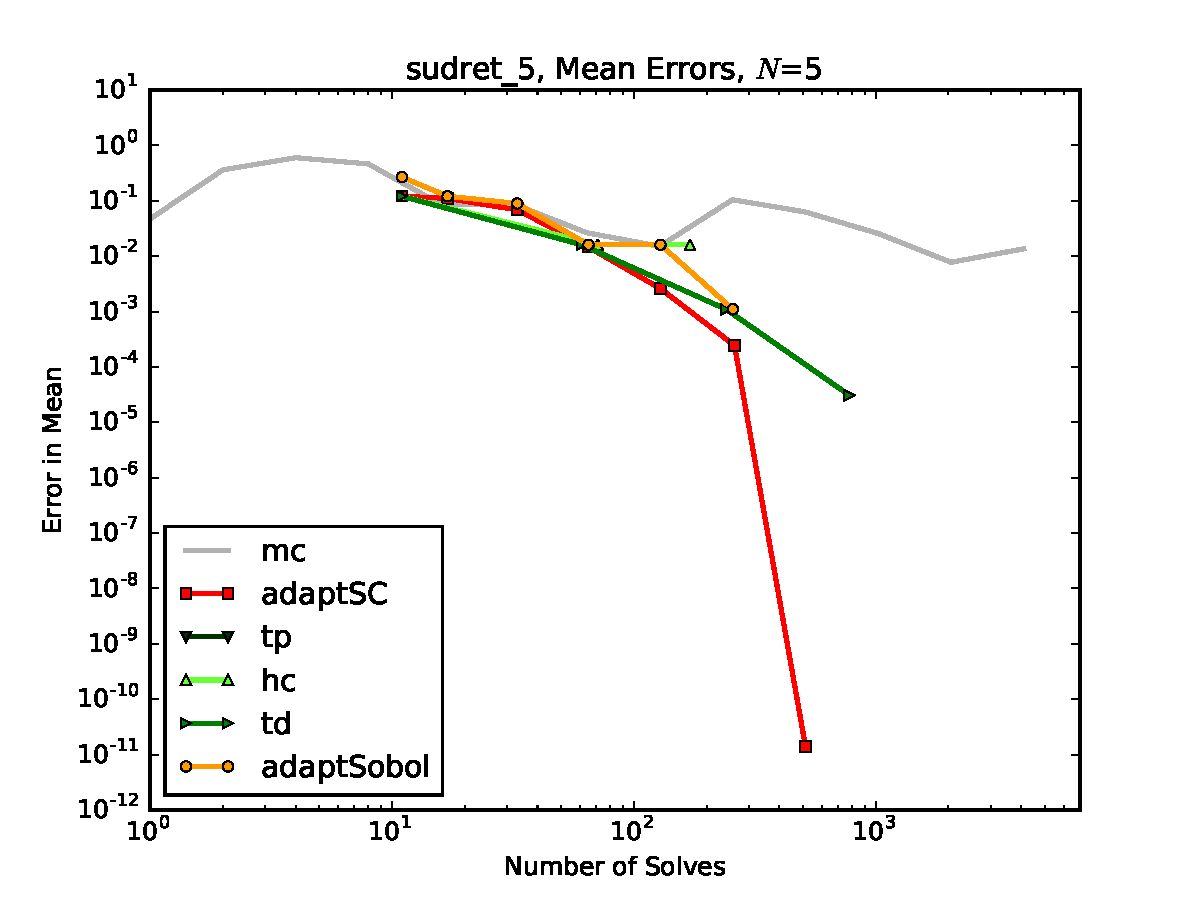
\includegraphics[width=0.7\linewidth]{anlmodels/sudret_5_mean_errs}
  \caption{Sudret Polynomial, $N=5$, Mean Convergence}
  \label{fig:sudretpoly mean errors 5}
\end{figure}
\begin{figure}[H]
  \centering
  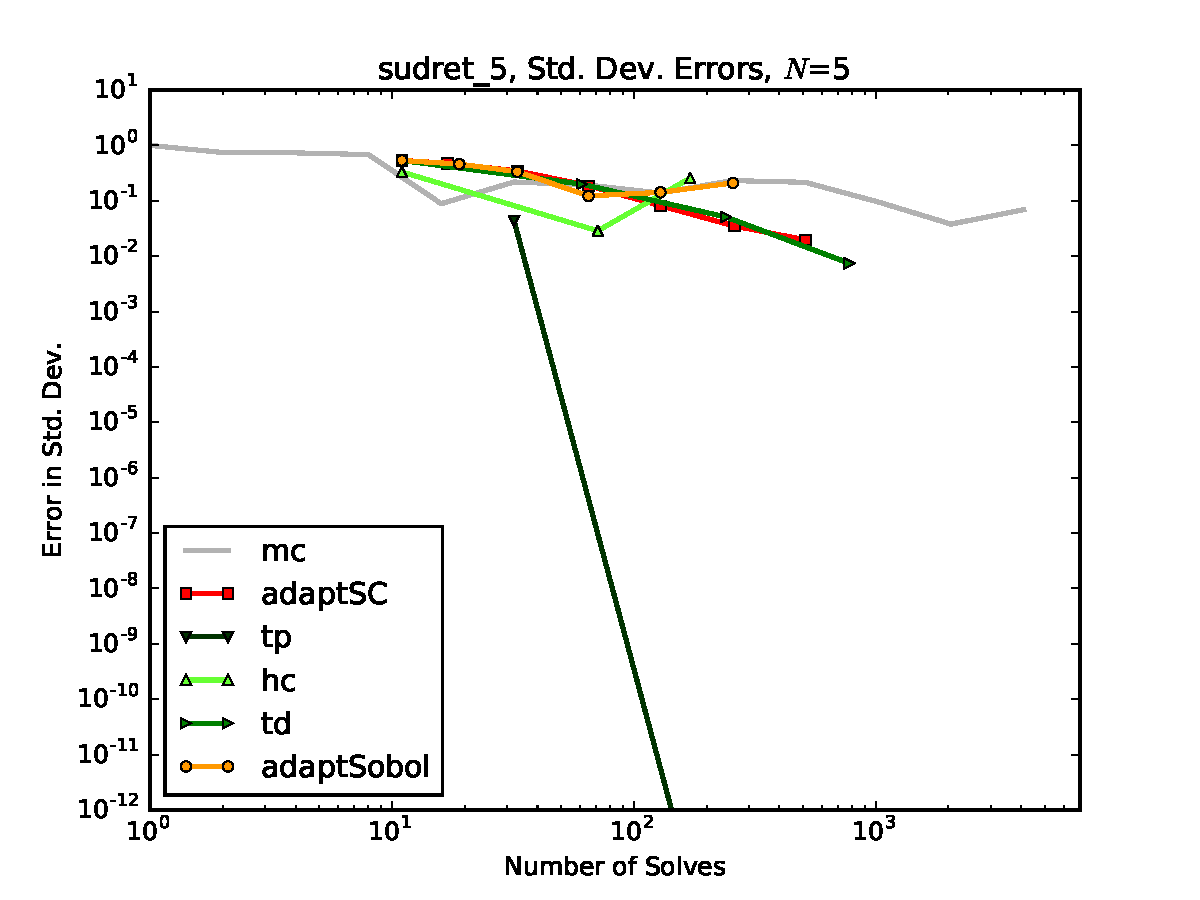
\includegraphics[width=0.7\linewidth]{anlmodels/sudret_5_variance_errs}
  \caption{Sudret Polynomial, $N=5$, Std. Dev. Convergence}
  \label{fig:sudretpoly var errors 5}
\end{figure}


\section{Attenuation}
This model is described in section \ref{mod:attenuation}.

\subsection{2 Inputs}
\begin{figure}[H]
  \centering
  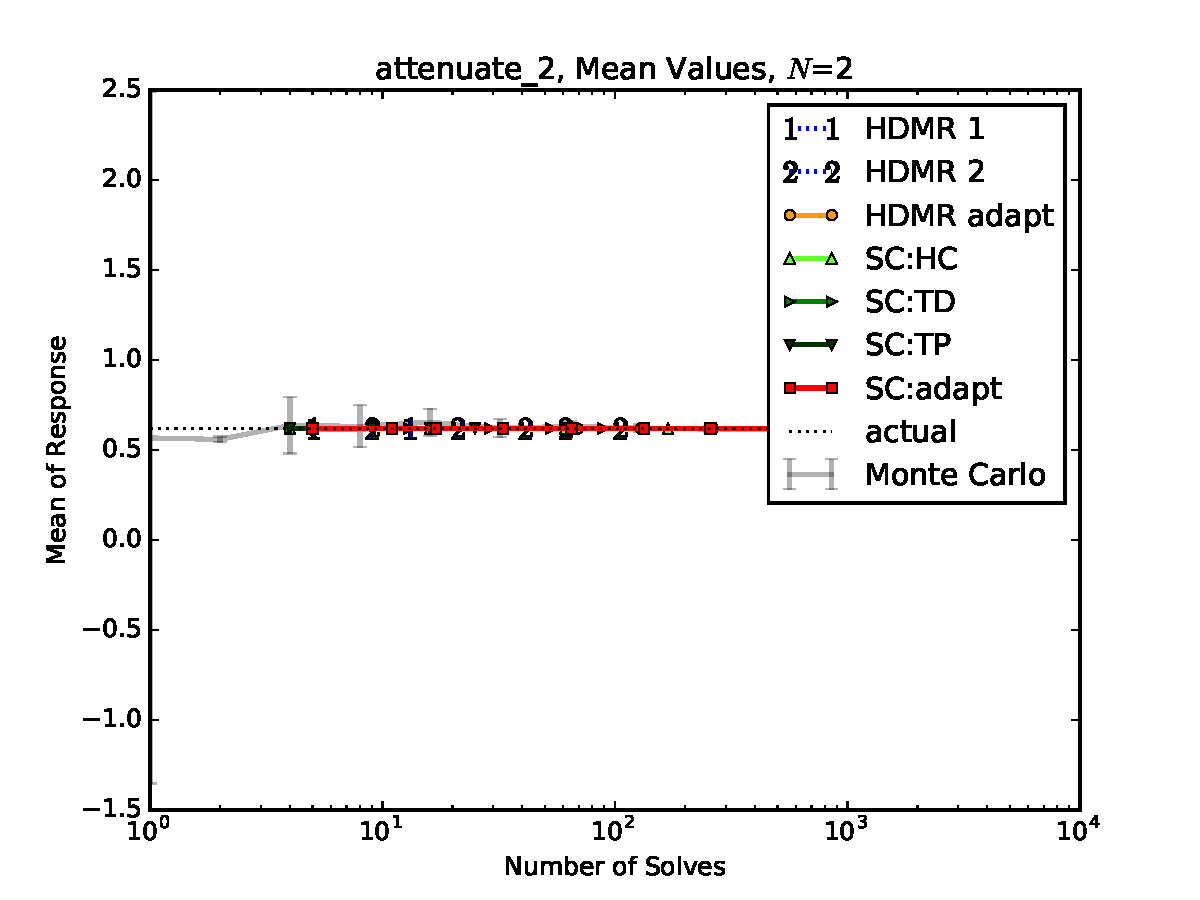
\includegraphics[width=0.7\linewidth]{anlmodels/attenuate_2_mean_vals}
  \caption{Attenuation, $N=2$, Mean Values}
  \label{fig:attenuate mean values 2}
\end{figure}
\begin{figure}[H]
  \centering
  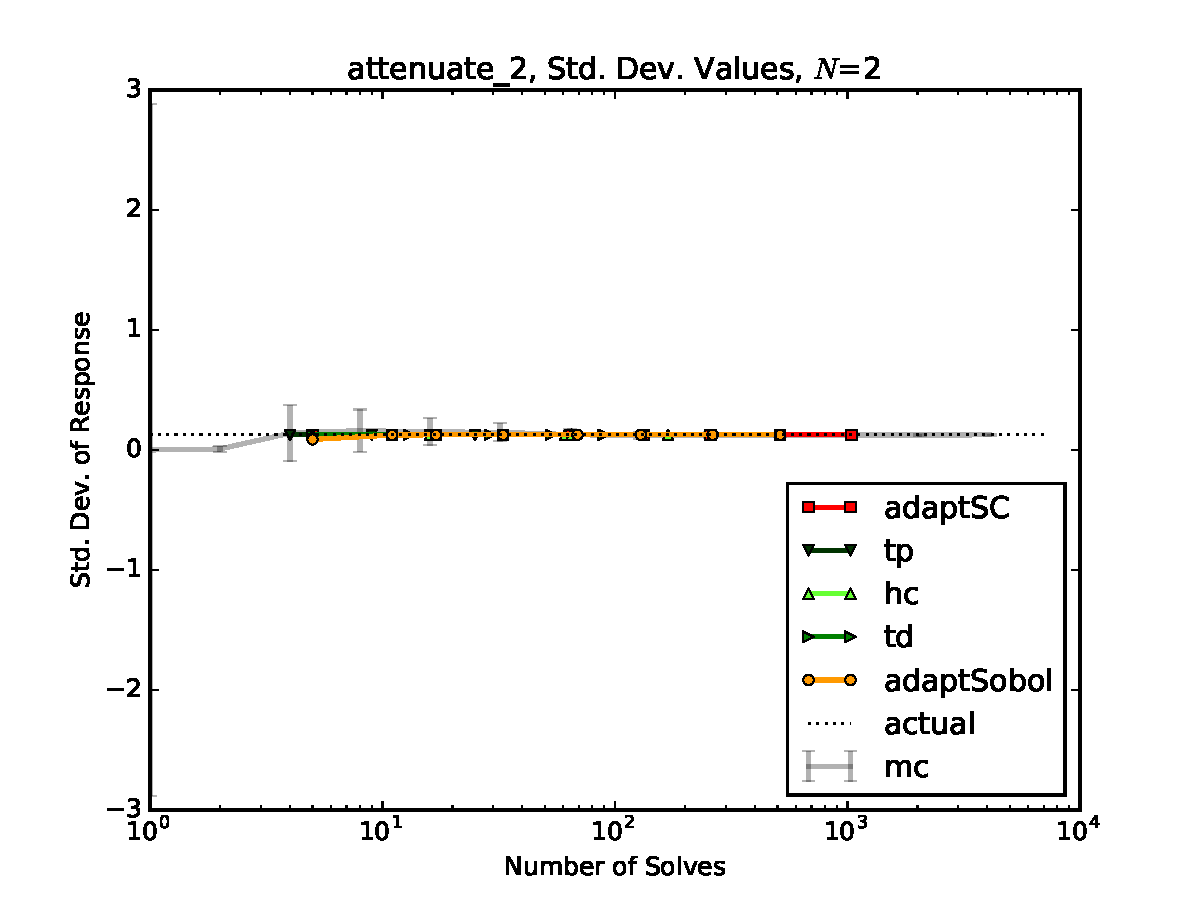
\includegraphics[width=0.7\linewidth]{anlmodels/attenuate_2_var_vals}
  \caption{Attenuation, $N=2$, Std. Dev. Values}
  \label{fig:attenuate var values 2}
\end{figure}

\begin{figure}[H]
  \centering
  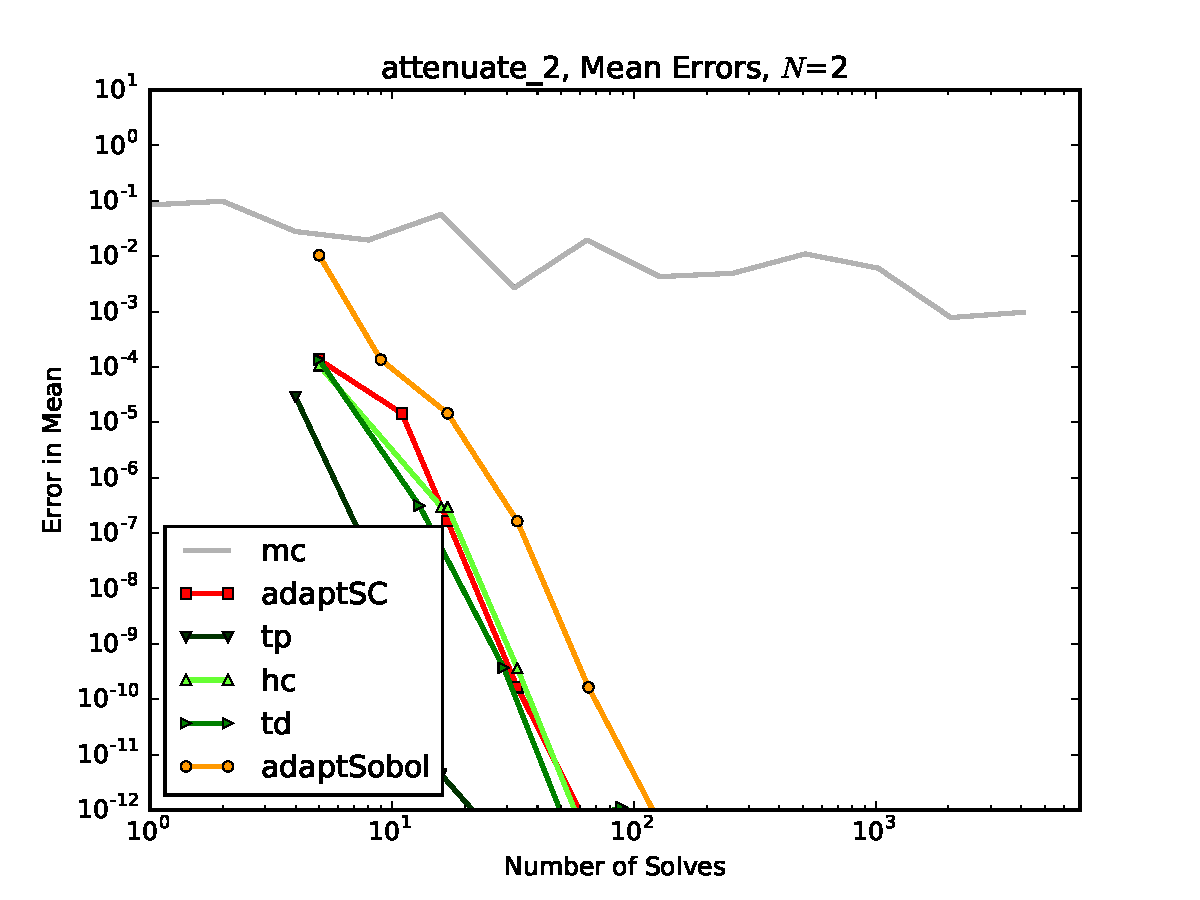
\includegraphics[width=0.7\linewidth]{anlmodels/attenuate_2_mean_errs}
  \caption{Attenuation, $N=2$, Mean Convergence}
  \label{fig:attenuate mean errors 2}
\end{figure}
\begin{figure}[H]
  \centering
  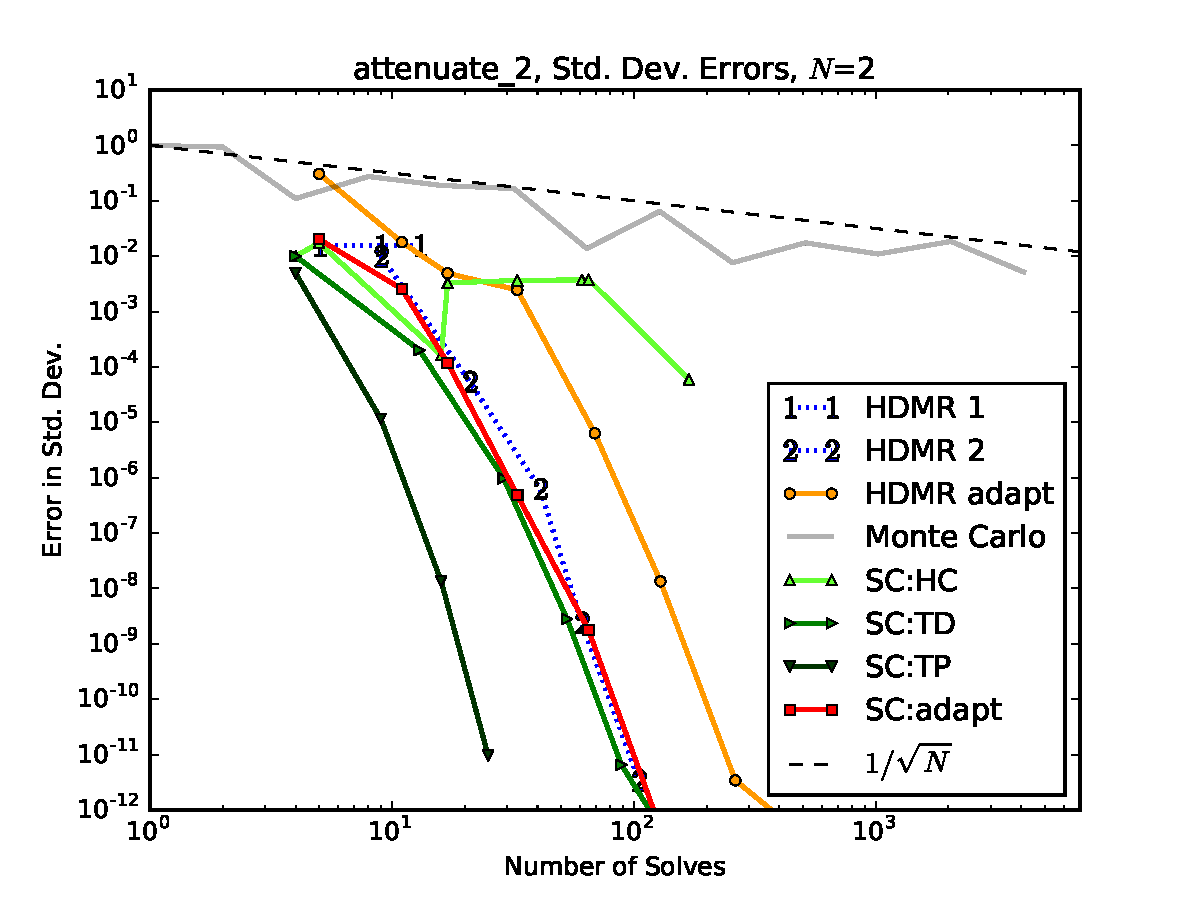
\includegraphics[width=0.7\linewidth]{anlmodels/attenuate_2_variance_errs}
  \caption{Attenuation, $N=2$, Std. Dev. Convergence}
  \label{fig:attenuate var errors 2}
\end{figure}


\subsection{4 Inputs}
\begin{figure}[H]
  \centering
  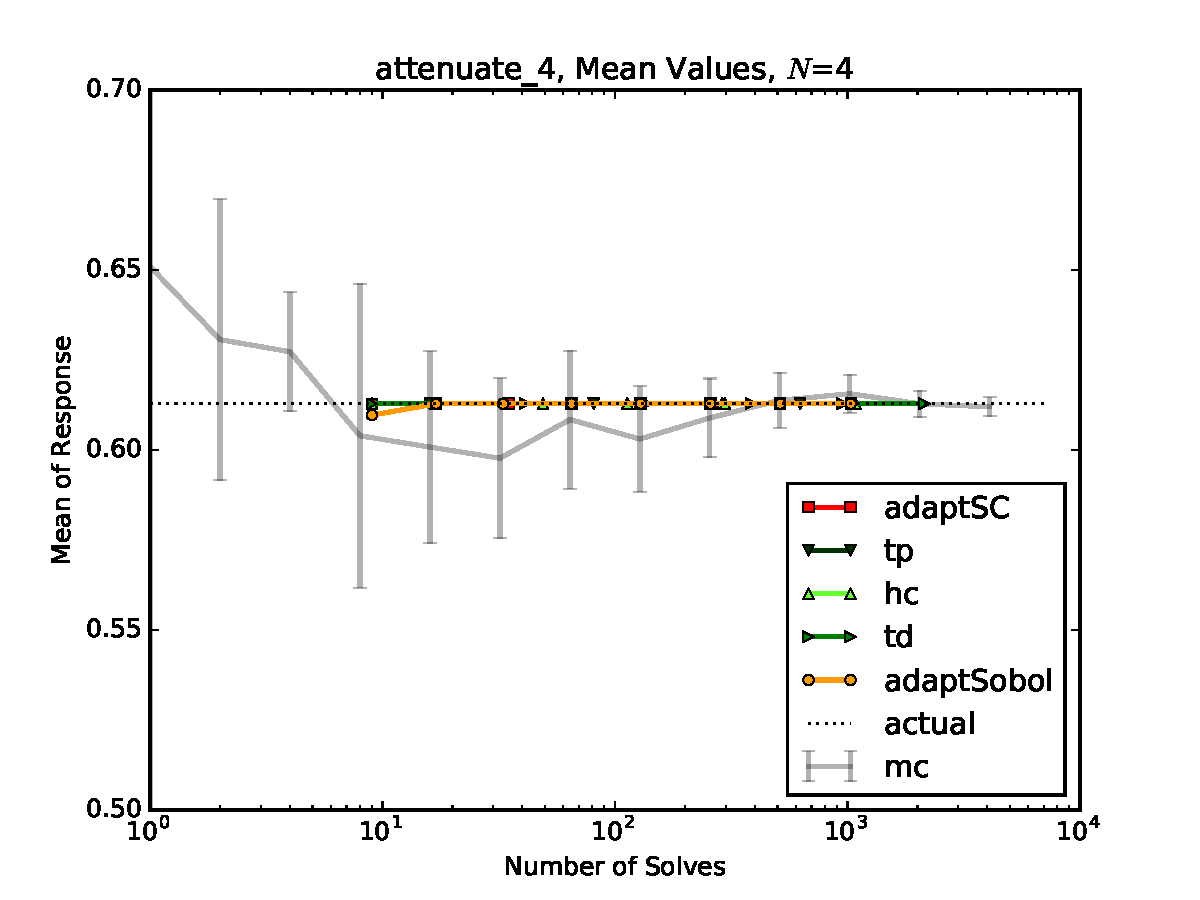
\includegraphics[width=0.7\linewidth]{anlmodels/attenuate_4_mean_vals}
  \caption{Attenuation, $N=4$, Mean Values}
  \label{fig:attenuate mean values 4}
\end{figure}
\begin{figure}[H]
  \centering
  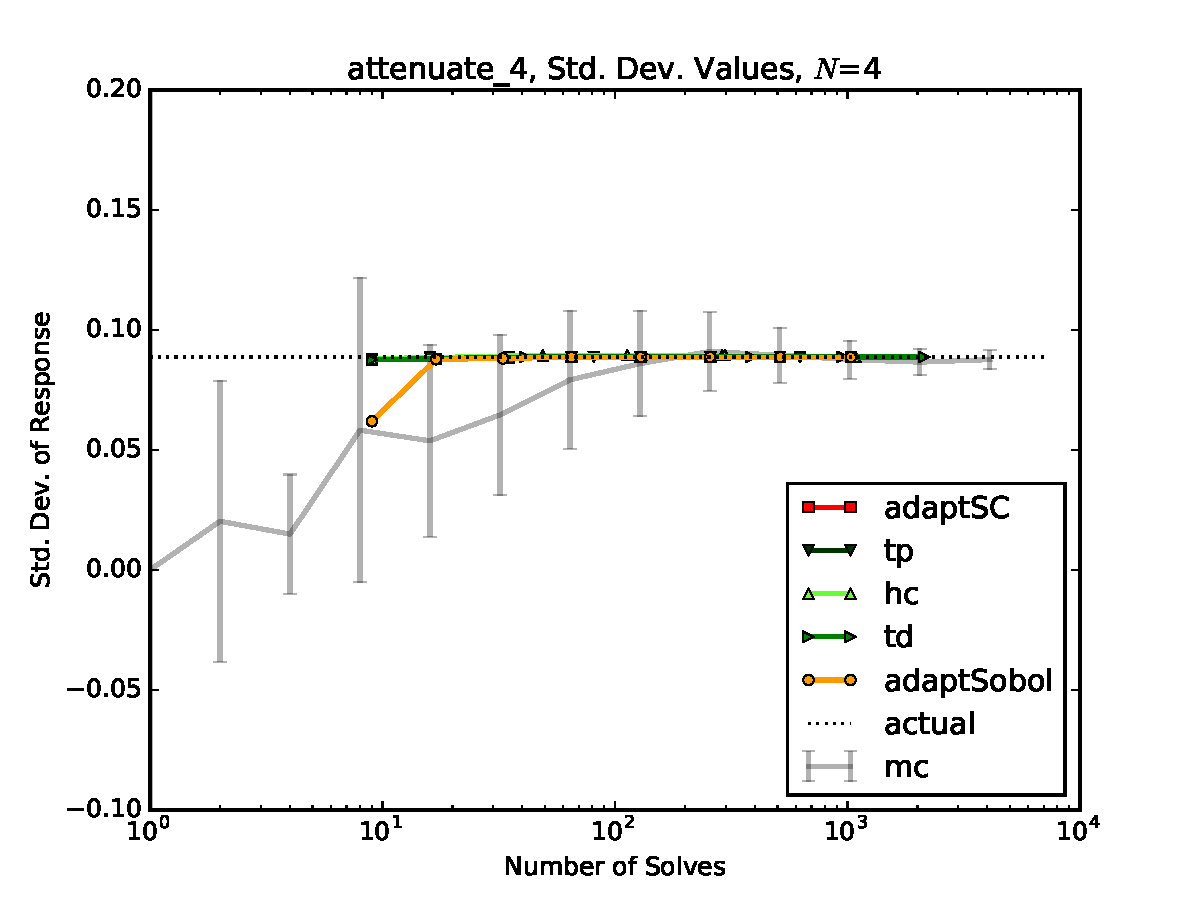
\includegraphics[width=0.7\linewidth]{anlmodels/attenuate_4_var_vals}
  \caption{Attenuation, $N=4$, Std. Dev. Values}
  \label{fig:attenuate var values 4}
\end{figure}

\begin{figure}[H]
  \centering
  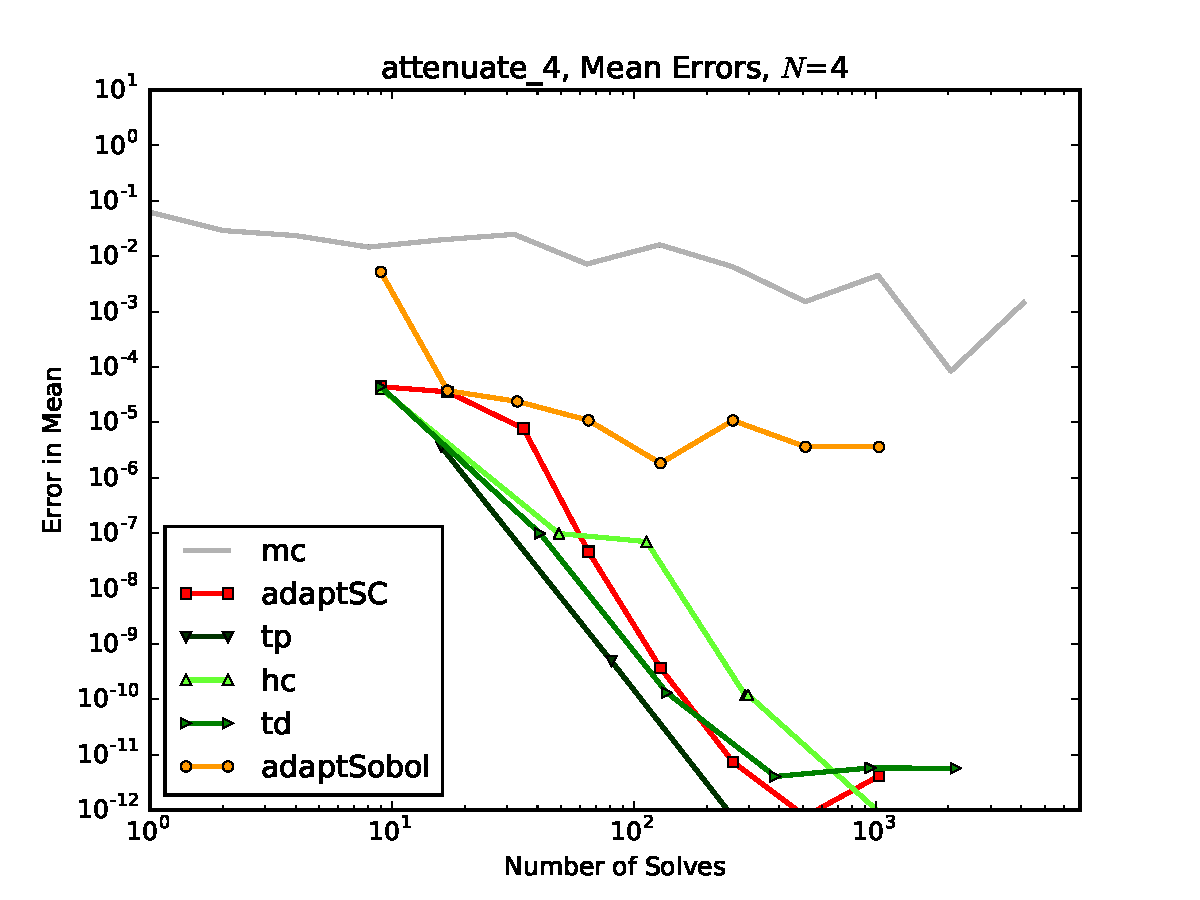
\includegraphics[width=0.7\linewidth]{anlmodels/attenuate_4_mean_errs}
  \caption{Attenuation, $N=4$, Mean Convergence}
  \label{fig:attenuate mean errors 4}
\end{figure}
\begin{figure}[H]
  \centering
  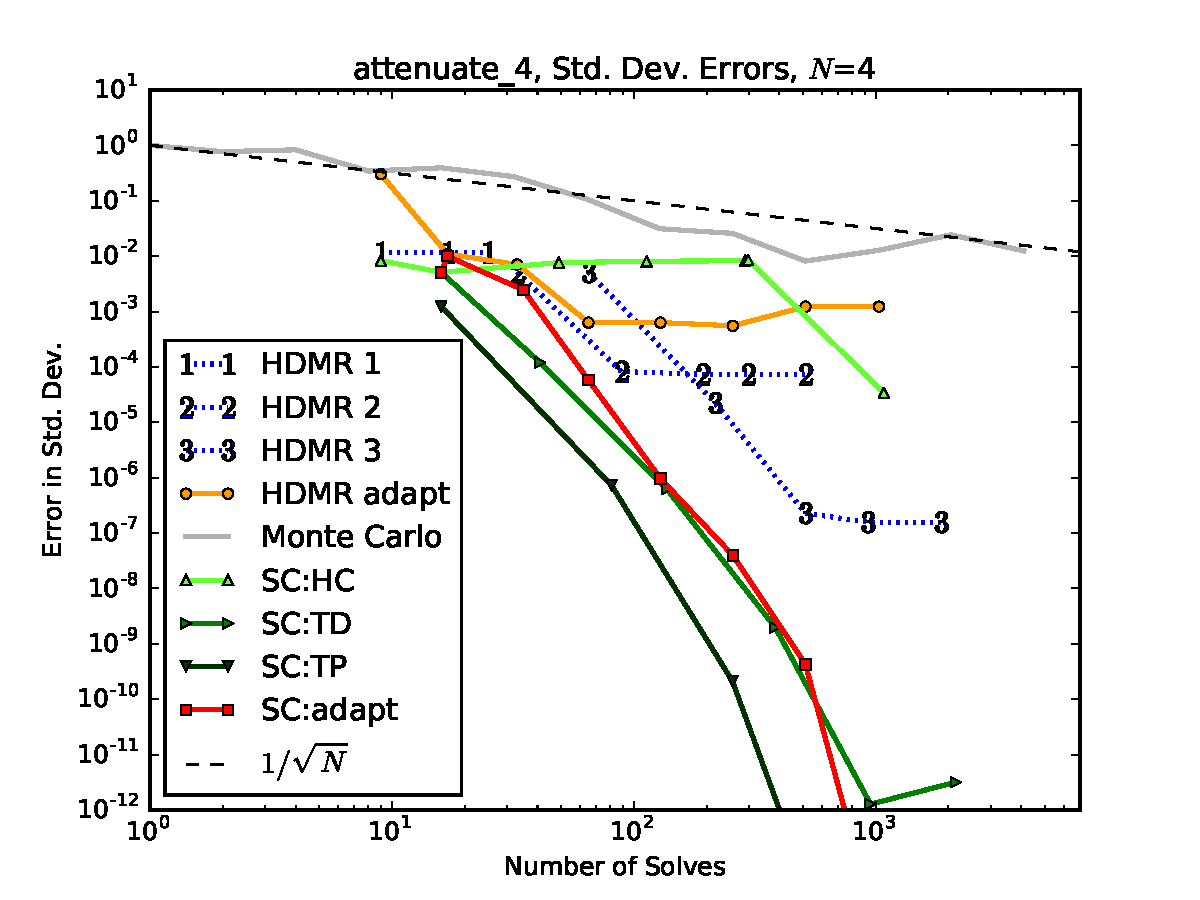
\includegraphics[width=0.7\linewidth]{anlmodels/attenuate_4_variance_errs}
  \caption{Attenuation, $N=4$, Std. Dev. Convergence}
  \label{fig:attenuate var errors 4}
\end{figure}

\subsection{6 Inputs}

\section{Gauss Peak}
This model is described in section \ref{mod:gausspeak}.


\section{Ishigami}
This model is described in section \ref{mod:ishigami}.

\section{Sobol G-Function}
This model is described in section \ref{mod:gfunc}.

\section{Anisotropic Polynomial}
This model is described in section \ref{mod:aniso}.
